%%%%%%%% ICML 2019 EXAMPLE LATEX SUBMISSION FILE %%%%%%%%%%%%%%%%%

\documentclass{article}

% Recommended, but optional, packages for figures and better typesetting:
\usepackage{microtype}
\usepackage{graphicx}
\usepackage{subfig}
\usepackage{booktabs} % for professional tables

% hyperref makes hyperlinks in the resulting PDF.
% If your build breaks (sometimes temporarily if a hyperlink spans a page)
% please comment out the following usepackage line and replace
% \usepackage{icml2019} with \usepackage[nohyperref]{icml2019} above.
\usepackage{hyperref}

% Attempt to make hyperref and algorithmic work together better:
\newcommand{\theHalgorithm}{\arabic{algorithm}}

% Use the following line for the initial blind version submitted for review:
\usepackage{icml2019}

% If accepted, instead use the following line for the camera-ready submission:
%\usepackage[accepted]{icml2019}

% The \icmltitle you define below is probably too long as a header.
% Therefore, a short form for the running title is supplied here:
\icmltitlerunning{System Identification through Expression Optimization}


%%%%%%%% this region contains all the stuff Anthony Added %%%%
\usepackage{bm}
\usepackage{amsfonts}
\usepackage{amsmath}
\newcommand{\todo}[1]{\textbf{[[#1]]}}
%%%%%%%%%%%%%%%%%%%%%%%%%%%%%%%%%%%%%%%%%%%%%%%%%%%%%%%%%%

\begin{document}

\twocolumn[
\icmltitle{System Identification through Expression Optimization}

% It is OKAY to include author information, even for blind
% submissions: the style file will automatically remove it for you
% unless you've provided the [accepted] option to the icml2019
% package.

% List of affiliations: The first argument should be a (short)
% identifier you will use later to specify author affiliations
% Academic affiliations should list Department, University, City, Region, Country
% Industry affiliations should list Company, City, Region, Country

% You can specify symbols, otherwise they are numbered in order.
% Ideally, you should not use this facility. Affiliations will be numbered
% in order of appearance and this is the preferred way.
\icmlsetsymbol{equal}{*}

\begin{icmlauthorlist}
\icmlauthor{Anthony Corso}{stanford}
\icmlauthor{Mykel Kochenderfer}{stanford}
\end{icmlauthorlist}

\icmlaffiliation{stanford}{Department of Aeronautics and Astronautics, Stanford University, Stanford, California, USA}

\icmlcorrespondingauthor{Anthony Corso}{acorso@stanford.edu}
\icmlcorrespondingauthor{Mykel Kochenderfer}{mykel@stanford.edu}

% You may provide any keywords that you
% find helpful for describing your paper; these are used to populate
% the "keywords" metadata in the PDF but will not be shown in the document
\icmlkeywords{Machine Learning, ICML}

\vskip 0.3in
]

% this must go after the closing bracket ] following \twocolumn[ ...

% This command actually creates the footnote in the first column
% listing the affiliations and the copyright notice.
% The command takes one argument, which is text to display at the start of the footnote.
% The \icmlEqualContribution command is standard text for equal contribution.
% Remove it (just {}) if you do not need this facility.

%\printAffiliationsAndNotice{}  % leave blank if no need to mention equal contribution
\printAffiliationsAndNotice{\icmlEqualContribution} % otherwise use the standard text.

\begin{abstract}
With the abundance of natural data from physical systems, much engineering and scientific value comes from an ability to discover the underlying, governing equations of a system, with little prior knowledge. Current approaches for data-driven system identification either find relationships in the data that aren't interpretable, or require significant prior knowledge from the user. This work describes a new approach to system identification that requires minimal user input and discovers governing equations that are parsimonious, generalizable and interpretable. This is enabled by recent advances in expression optimization, allowing for the automated discovery of mathematical expressions from a combinatorically large set of possibilities. Using simulated data, our approach correctly identifies both linear and nonlinear PDEs including the Navier-Stokes equations. It can also generate exact and approximate Koopman eigenfunctions for nonlinear ODEs. The ability to interpret large amounts of data will allow researchers to better understand and control important natural systems, such as the earth’s climate, for addressing global warming and fluid flow for more efficient energy generation and transportation.
\end{abstract}

\section{Introduction}
\label{introduction}

Over the past several decades machine learning and artificial intelligence have made great strides in learning patterns from large amounts of data. Although accurate, these systems are often uninterpretable by the human researchers who create them. They do not report an explanation for their predictions nor do they generalize well when the task is changed slightly.

Recently, however, strides have been made to create AI systems that, rather than just looking for trends, look for causal explanations of observed data (Bridewell, 2008, Brunton, 2016). If an AI system can correctly determine a simple underlying model for a system, then it can provide an explanatory account of the data and generalize in predicting behavior under a wider variety of conditions. This can help researchers more quickly discover models that explain experimental data.

\todo{Describe the current systems and there limitations. Specifically that system identification approaches fall into two categories 1) Those that require no user input but produce opaque results 2) Those that produce interpretable results but require lots of prior knowledge}

The goal of this work was to create a system that could discover, from data, the governing equations or Koopman eigenfunction of a dynamical system. The system should require minimal prior knowledge from the user, be robust to noise and operate on small amounts of data. This paper is organized as follows. Section \ref{systemidentification} describes how governing equations could be derived from data as well as the connection between equation discovery and the approximation of the Koopman operator. Section \ref{sieo} details the approach known as system identification through expression optimization (SIEO) and section \ref{results} reports the results of SIEO applied to four model systems. Finally, section \ref{conclusion} concludes and discusses directions for future investigation. 



\section{System Identification}
\label{systemidentification}

The goal in system identification is to find a parsimonious description of a dynamical system using data. This section will outline some of the previous work on system identification, and then discuss the two forms of identification that are the focus of this work.

\subsection{Past Approaches}
\todo{
\begin{itemize}
    \item SINDy and HPM where you have to specify entire features
    \item DMD/POD where you get a low dimensional approximation without much user input but the resulting modes don't make contact with domain concepts.
    \item extended DMD for Koopman approximation (need to specify features)
\end{itemize}}

\subsection{Governing Equations}
One approach to understanding a dynamical system is to determine its underlying governing equations. If the system is a spatio-temporal process, then governing equation can be written as partial differential equation (PDE) of the form
\begin{equation}
    \frac{\partial x (\vec{r},t)}{\partial t} = \theta_1 g_1(x(\vec{r},t)) + ... + \theta_n g_n(x(\vec{r},t))
\end{equation}
where $\vec{r}$ are the spatial dimension, $x$ is a state variables, $g_i$ are feature functions and $\theta_i$ are the corresponding coefficients. Given a mapping $g_i$, and a state $x$, the coefficients of the PDE can be found via a linear model of the form 
\begin{equation}
 y = \theta^T \tilde{x}
 \end{equation}
where $y = \partial u/ \partial t$ and $\tilde{x} = \begin{bmatrix}g_1(u), & \hdots, & g_n(u) \end{bmatrix}^T$. A good approximation of $\theta^T$ can be found by sampling many $y$ and $\tilde{x}$ points and then performing multiple linear regression. The goal, then, is to find the optimal set of features $g_i$ (and corresponding $\theta_i$) for producing the best fit between $y$ and $\tilde{x}$.

Note that when discovering a governing equation, only the input data is transformed by a nonlinear mapping, while the output data remains unchanged. If a nonlinear mapping were found that could be applied to both the input and output, then it would be possible to convert a nonlinear system into a linear one. This is known as finding the Koopman operator of a system and it is discussed in the next section.

\subsection{Koopman Operators}
Nonlinear dynamical systems are far more challending to understand and control than their linear counterparts. One promising area of analysis is Koopman theory [CITATION] which states that any nonlinear dynamical system can be converted into a linear system under the state-space mapping
\begin{equation}
x \rightarrow \vec{g}(x)
\end{equation}
where $\vec{g}(x) = \begin{bmatrix} g_1(x), g_2(x), & \hdots \end{bmatrix}^T$ are the Koopman eigenfunctions. In general, $\vec{g}$ is infinite dimensional and therefore it must be approximated with a finite-dimensiona mapping.

The Koopman operator can take a nonlinear dynamical system of the form
\begin{equation}
\vec{x}^{t+1} = \vec{f}(\vec{x}^t)
\end{equation}
and transform it into the linear system
\begin{equation}
\label{fig:linsys}
\vec{g}(x)^{t+N} = K^N \vec{g}(x)^{t}
\end{equation}
Thus, if the the Koopman operator is known, all of the mathematical technologies developed around linear systems can be brought to bear on a nonlinear system. 

If the Koopman eigenfunctions contain the identity function $g(x) = x$ then the Koopman operator is said to be \emph{state-inclusive} and the un-transformed state of the system can be found directly from the linear system (\ref{fig:linsys}), without finding an inverse transformation $\vec{g}^{-1}$.

Given a finite approximation to the Koopman eigenfunctions $\vec{g}(x) = \begin{bmatrix} g_1(x), & \hdots, & g_n \end{bmatrix}^T$, the matrix $K$ can be found via a linear model of the form 
\[ y = K \tilde{x} \]
where $y = \vec{g}(x^{t+1})$ and $\tilde{x} = \vec{g}(x^t)$. If many points are sampled for $y$ and $\tilde{x}$ then multiple linear regression can provide the least-squares estimate of $K$. The goal for approximating the Koopman operator is to find finite approximation $\vec{g}(x)$ that creates the best fit between $y$ and $\tilde{x}$.

It should now be clear that the problems of equation discovery and approximating the Koopman operator are identical except for the transformation of the output data in the latter case. The next section describes a new approach to finding these nonlinear mappings from the vast number of possibilities.

\section{System Identification through Expression Optimization (SIEO)}
\label{sieo}
The process of discovering a nonlinear mapping for system identification from data has three steps.
\begin{enumerate}
    \item Define a set of nonlinear features
    \item Define a loss function to measure the success of a group of features (referred to as a \textit{mapping})
    \item Search through the possible mappings to find the optimal
\end{enumerate}
The first and third task each involve searching through a combinatorically large set of possibilities and therefore pose a substantial computational challenge. The next subsection discusses how the first task can be performed efficiently using a context-free grammar. The next subsection describes two useful loss functions for the two system identification tasks. The last section describes a search technique that combines expression optimization with a greedy heuristic search for finding the optimal mapping. The combination of these techniques comprise the  approach known as System Identification through Expression Optimization (SIEO).

\subsection{Context-Free Grammar}

% Motivate the need for a grammar
There are an infinite number of features that could make up a mapping, but, researchers don't generally know a priori which features will be good candidates. Thus, a design goal of SIEO is to require minimal prior knowledge from the user while still constraining the possible features to be searched.

% Describe what the grammar is
To this end, SIEO relies on a domain-specific \textit{grammar}, provided by the user, that gives the rules for generating feature functions. A grammar is a set of production rules that govern a language (or a set of expressions). Each rule can either be \textit{non-terminal}, in which the rule relates generic expressions together (e.g. multiplication), or \textit{terminal}, in which an expression is concretely defined (e.g. the observed data). Each expression in the language can be represented by a tree of operators, each of which is part of the grammar. Once a grammar is defined, expressions can be sampled from the grammar with varying levels of complexity (as defined by the depth of the expression tree).

% Given an example of a sample from the grammar
For example, the grammar in figure \ref{fig:advdifgrammar} has rules for differentiation, multiplication, and division. Sampling from a grammar is a process of selecting production rules and then filling in any non-terminal expressions until only terminal expressions remain. For example, in the expression 
\begin{equation}
    u \frac{\partial u}{\partial x }
\end{equation}
the first (non-terminal) production rule chosen is multiplication. Then, on the left side, the terminal expression $u$ was chosen, and on the right side, the non-terminal derivative rule was chosen, followed by the terminal expression $u$. Grammars define a constrained, but still infinite, set of possible expressions which can be made finite be specifying a maximum expression depth for a grammar. 

The benefit to this approach is two-fold
\begin{enumerate}
    \item For the cost of defining a simple grammar, an infinite number possible expressions (ranging from simple to complex) can be produced
    \item The researcher can encode into the grammar any information she may have regarding relationships between the input and output data.
\end{enumerate}
As will be demonstrated in later sections, many familiar PDEs have features that come from a very simple grammar (2-3 rules) with a very short depth (2-3). The next subsection describes the loss functions used to compare different features.  

\subsection{Choice of Loss Function}
\label{lossfunction}
When attempting to discover a governing equation to explain data, the object is to find a mapping that describes the output data well, but also to find a mapping that is simple (i.e. has fewer features). To balance this multi-objective, the negative adjusted $R^2$ value ($R_{\rm adj}^2$) of the fit was used for the loss function. The traditional $R^2$ value always increases when new features are added so it makes our algorithm susceptible to overfitting. $R_{\rm adj}^2$, however, penalizes the addition of more features via [CITATION]
\[R_{\rm adj}^2 = R^2 - \alpha (1-  R^2)(n-1)\]
where $n$ is the number of features in the model. Note that when $n=1$, this expression reduces to the traditional $R^2$ value. But when $n>1$, then the difference between $R^2$ and 1 is scaled by the number of parameters. Thus, as a rule of thumb, $\alpha \in [0, \infty)$ should be large when you expect there to be excellent agreement between the input and output (i.e. for synthetic, noise-free data) and should be closer to 0 when near-perfect agreement is not expected (i.e. real world data). The loss function is explicitly defined as 
\begin{equation}
    l_R(\theta, \vec{g}) = - R_{\rm adj}^2(\theta, \vec{g})
\end{equation}

For the goal of discovering Koopman eigenfunctions, however, parsimony is no longer a consideration so a new loss function needs to be used. Given a linear system with $n_g$ number of Koopman eigenfunctions, the loss function associated with the Koopman operator $K \vec{g}$ is given by

\[ l_k(K \vec{g}) = \frac{1}{n_g}||\vec{g}(\vec{x})^{t+1} - K \vec{g}(\vec{x})^{t}||_2^2 \]

The scaling by $1/n_g$ is so that that algorithm does not get penalized for adding more Koopman eigenfunctions to approximate the nonlinear system, and instead focuses on closely matching each new state variable on each iteration. This loss function is referred to as the \emph{average sum of squares}. The following subsection ties together the use of a grammar and the loss functions to explain how expression optimization and heuristic search are used to select features.


\subsection{Feature Selection Algorithms}

The problem of selecting from a group of possible features is a challenging one. If there are $N$ possible features then there are $2^N$ possible subsets to pick from. It is infeasible to search the entire space of combinations for even moderate values of $N$, so heuristic searches need to be employed. 

Previous approaches have used sparsity-promoting regression techniques such as LASSO [Citation] but these approaches are brittle when the input data suffers from mulicollinearity [ PDE citation]. In this work, the heuristic that performed the best was a modified form of a greedy search algorithm that combined both forward and backward search. The high-level structure of the algorithm is given in Algorithm \ref{alg:featureselection}.

The algorithm starts by performing a greedy forward search (Algorithm \ref{alg:forwardsearch}), where, on each iteration, a feature is greedily added to the mapping until there is either no further improvement or a specified threshold is hit. Then, the feature selection algorithm performs a greedy backward search on the mapping (Algorithm \ref{alg:backwardsearch}), where features are removed if their absence reduces the loss function. This entire process iterates until there is no further improvement of the mapping, at which point it is returned.

\begin{algorithm}[tb]
   \caption{Feature Selection}
   \label{alg:featureselection}
\begin{algorithmic}
   \STATE {\bfseries Input:} Loss function $l_f$, \\
   \quad \quad \quad New feature generator $n_f$, \\
   \quad \quad \quad Threshold $t$ \\
   \STATE Initialize $mapping = [ \ ]$
   \REPEAT
   \STATE $old\_mapping = mapping$
   \STATE $mapping = {\rm forward\_search}(mapping, lf, n_f, t)$
   \STATE $mapping = {\rm backward\_search}(mapping, lf, n_f, t)$
   \UNTIL $old_mapping == mapping$
\end{algorithmic}
\end{algorithm}

\begin{algorithm}[tb]
   \caption{Forward Search}
   \label{alg:forwardsearch}
\begin{algorithmic}
   \STATE {\bfseries Input:} Loss function $l_f$, \\
   \quad \quad \quad Current mapping $mapping$, \\
   \quad \quad \quad New feature generator $n_f$, \\
   \quad \quad \quad Threshold $t$ \\
   \STATE Initialize $lowest = l_f(mapping)$
   \REPEAT
   \STATE $mapping = {\rm concat}(mapping, \ n_f(mapping))$
   \IF{$l_f(mapping) < lowest$}
   \STATE $lowest = l_f(mapping)$
   \ELSE
   \STATE {\bfseries return} $mapping$
   \ENDIF
   \UNTIL $lowest < t$
\end{algorithmic}
\end{algorithm}

\begin{algorithm}[tb]
   \caption{Backward Search}
   \label{alg:backwardsearch}
\begin{algorithmic}
   \STATE {\bfseries Input:} Loss function $l_f$, \\
   \quad \quad \quad Current mapping $mapping$, \\
   \quad \quad \quad Threshold $t$ \\
   \STATE Initialize $lowest = l_f(mapping)$
   \REPEAT
   \STATE Initialize $losses = [ \ ]$
   \FOR{$feat$ {\bfseries in} $mapping$}
   \STATE $new\_mapping = {\rm remove}(mapping, feat)$
   \STATE ${\rm push}(losses, l_f(new\_mapping))$
   \ENDFOR
   \STATE $i = {\rm arg\,max}(losses)$
   \IF{$losses[i] < lowest$}
   \STATE $lowest = losses[i]$
   \STATE $mapping = {\rm remove}(mapping, feat)$
   \ELSE
   \STATE {\bfseries return} $mapping$
   \ENDIF
   \UNTIL $lowest < t$
\end{algorithmic}
\end{algorithm}

The substantial missing piece of this process is how to find the next feature to add to the list. As described previously, a comprehensive search is infeasible, so an expression optimization technique must be used.


\subsubsection{Expression Optimization}
There are several excellent algorithms for expression optimization using a grammar, but the one used in SIEO is  Grammatical Evolution (GE), an expression optimization approach introduced by [CITATION]. Each feature that is sampled from the grammar is expressed as an unbounded integer array that can be parsed from left to right into an expression tree. Each integer array is transformed in a manner similar to genetic algorithms. The basic operations are
\begin{enumerate}
\item \textbf{Selection} - The integer arrays with the best fitness (lowest loss function) are selected from the population
\item \textbf{Crossover} - The fittest individuals produce offspring that carry traits from the parents
\item \textbf{Mutation} - The integer arrays are randomly altered (while preserving the rules of the grammar)
\item \textbf{Gene Duplication} - Where useful genes are copied in the integer array so that they are less likely to be lost
\item \textbf{Pruning} - Some integer arrays will contain genetic information that is unused (put there through crossover). So with some probability unused genes are pruned in an individual.
\end{enumerate}

These operations are applied to a large number of individuals over many generations in order to produce optimal features from the large space of possibilities. In the following section, SIEO is applied to several model systems to demonstrate several possible applications.


\section{Results}
\label{results}
SIEO was tested on four separate model problems to demonstrate its capabilities and probe its robustness. The first two problems are equation discovery for PDEs. The first is used to demonstrate that SIEO can operate with limited and noisy data. The second is to demonstrate that the algorithm scales to problems with multiple spatial dimensions and multiple state variables. The next two model systems show the utility of SIEO for approximating Koopman functions, first, by finding them exactly and then by finding a good finite approximation.

\subsection{Advection-Diffusion Equation}

The first model problem is the unsteady 1D advection-diffusion equation which describes the general linear transport of material $u$ in a fluid. The governing equation has the form 
\begin{equation} 
\frac{\partial u}{\partial t} = D\frac{\partial^2 u}{\partial x^2} - v \frac{\partial u}{\partial x}
\end{equation}
where $D$ is the diffusion coefficient, $v$ is the fluid velocity. Synthetic data is generated using the exact solution derived by [Van Genuchten citation 1982] which for boundary conditions 
\begin{align}
  u(x,0) &= u_0 \\
  u(0,t) &= u_L \\
  \frac{\partial u}{\partial x}(\infty, t) &= 0
\end{align}
is found to be 
\begin{equation}
  \begin{split}
  u(x,t) = u_0 + \frac{1}{2}&(u_L - u_0) \left({\rm erfc}\left[ \frac{x - vt}{2\sqrt{Dt}}\right]\right. \\
  &+ \left.{\rm exp}(vx/D) {\rm erfc}\left[ \frac{x + vt}{2\sqrt{Dt}}\right] \right)
  \end{split}
\end{equation}
This solution is plotted in figure \ref{fig:advdif} for $x>0$, $t>0$, $D=1$, $v=1$, and $U_L = 1$.

\begin{figure}
\vskip 0.2in
\begin{center}
\centerline{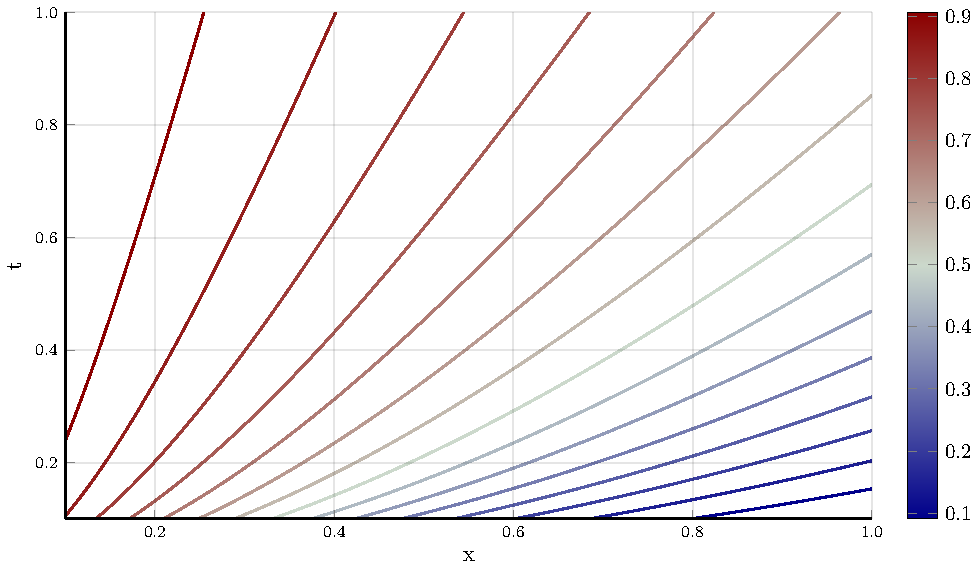
\includegraphics[width=\columnwidth]{./figures/advdif}}
\caption{Unsteady data from the 1D advection-diffusion equation}
\label{fig:advdif}
\end{center}
\vskip -0.2in
\end{figure}

To apply SIEO the exact solution was sampled at 200 temporal points in the range $t = (0, 0.1)$ and between 10 and 200 spatial points . Then, additive white Gaussian noise at a level $\eta \in (0, 0.2)$ was added to the data such that the standard deviation of the noise is given by $\sigma = \eta \ {\rm std}(u)$. The grammar shown in figure \ref{fig:advdifgrammar} was used for the expression optimization routine and was limited to a tree depth of 3. The adjusted $R^2$ loss function was used with the parameter $\alpha = 0.5$. The solution was denoised using total variation filtering [tv citation] both before and after the numerical differentiation.
\begin{figure}
    \vskip -0.2in
    \centering
    \begin{equation*}
    \begin{split}
    \mathbb{R} &\mapsto u \\
    \mathbb{R} &\mapsto \frac{d\mathbb{R}}{dx} \\
    \mathbb{R} &\mapsto \mathbb{R} \times \mathbb{R} \\
    \mathbb{R} &\mapsto \mathbb{R} / \mathbb{R}
    \end{split}
    \end{equation*}
    \vskip -0.15in
    \caption{Grammar used for the advection-diffusion equation}
    \label{fig:advdifgrammar}
    \vskip -.15in
\end{figure}
The results of six test cases are shown in table \ref{tab:advdifresults}. After the trial number, the first two columns show the number of spatial sample points used and the noise level, respectively. The last two columns show the percent error in the model parameters, $v$ and $D$ when compared to their exact values. In all six test cases, SIEO determined the correct form of the governing equation. When the noise is 1-5 \% and the number of sample points is 35 or larger, the error in the parameters remains small. In the two most challenging test cases (trials 3 and 6), the fit parameters $v$ and $D$ show high levels of error but the correct form the equation was still discovered accurately which demonstrates the robustness of SIEO to find an accurate and generalizable model with large amounts of noise or limited data.

\begin{table}[t]
\caption{Error in solution parameters for different noise levels and spatial resolutions}
\label{tab:advdifresults}
\vskip 0.15in
\begin{center}
\begin{small}
\begin{sc}
\begin{tabular}{lccccr}
\toprule
 & Sample &  & Error & Error\\
Trial & Points & Noise & in $v$ & in $D$\\
\midrule
1 & 200 & 1\%  & 0.78 \% & 1.54 \% \\
2 & 200 & 5\%  & 5.64 \% & 2.84 \% \\
3 & 200 & 20\%  & 30.12 \% & 6.60 \% \\
4 & 100 & 0\%  & 0.84 \% & 0.29 \% \\
5 & 35 & 0\%  & 6.38 \% & 2.21 \% \\
6 & 10 & 0\%  & 1.19 \% & 19.02 \% \\
\bottomrule
\end{tabular}
\end{sc}
\end{small}
\end{center}
\vskip -0.1in
\end{table}


\subsection{Navier-Stokes Equations}
The second test system is the incompressible 2D Navier-Stokes equations which describe the motion of a viscous fluid. The Navier-Stokes equations are given by
\begin{align}
  \frac{\partial u}{\partial x} + \partial{v}{\partial y} &= 0 \\
  \frac{\partial u }{\partial t} + u \frac{\partial u }{\partial x} + v \frac{\partial u }{\partial y} &= - \frac{1}{\rho} \frac{\partial p}{\partial x} + \frac{\mu}{\rho}\left( \frac{\partial^2 u}{\partial x^2} + \frac{\partial^2 u}{\partial y^2} \right) \\
\frac{\partial v }{\partial t} + u \frac{\partial v }{\partial x} + v \frac{\partial v }{\partial y} &= - \frac{1}{\rho} \frac{\partial p}{\partial v} + \frac{\mu}{\rho}\left( \frac{\partial^2 v}{\partial x^2} + \frac{\partial^2 v}{\partial y^2} \right)
\end{align}

where $\rho$ is the fluid density, $(u, v)$ is the fluid velocity, $p$ is the pressure, and $\mu$ is the viscosity. The first equation represents the conservation of mass and the next two equations represent conservation of momentum in the $x$ and $y$ directions, respectively. These equations are nonlinear, have multiple dimensions ($x$ and $y$) and multiple degrees of freedom ($u$, $v$, and $p$), which makes them a challenging model system to identify.

Synthetic data was collected from the simulation of vortex shedding behind a circular cylinder at a Reynold's number of 50. The simulation was performed using \emph{PyFR} [citation] and 10 snapshots were taken with a timestep of $dt = 0.001$, $M = 0.2$ and $\rho \approx 1$ (with a very small amount of compressibility in the solution). A single frame of the simulation is shown in figure \ref{fig:ns_data}, with $u$, $v$, and $p$ on separate plots. The grammar in figure \ref{fig:nsgrammar} was used to produce features up to a depth of 3, yielding 363 features and $2^{363}$ expressions to be searched.

\begin{figure}
  \vskip 0.2in
    \subfloat[$x$-velocity]{\label{xvelocity}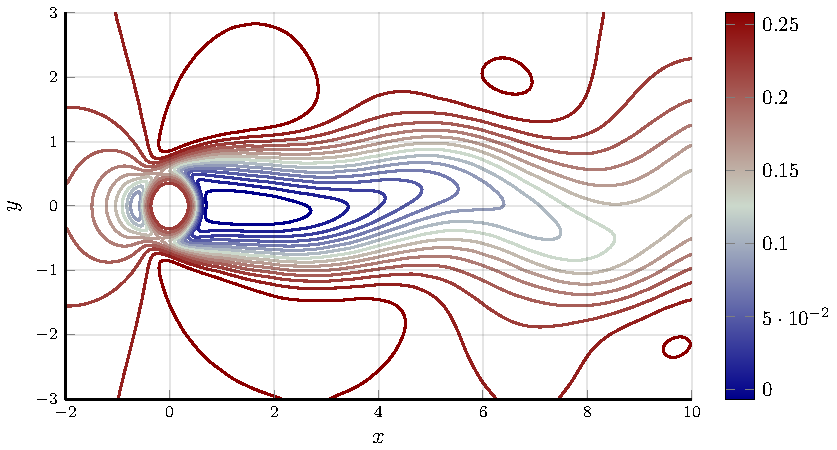
\includegraphics[width=\columnwidth]{./figures/xvel}} \\
    \subfloat[$y$-velocity]{\label{yvelocity}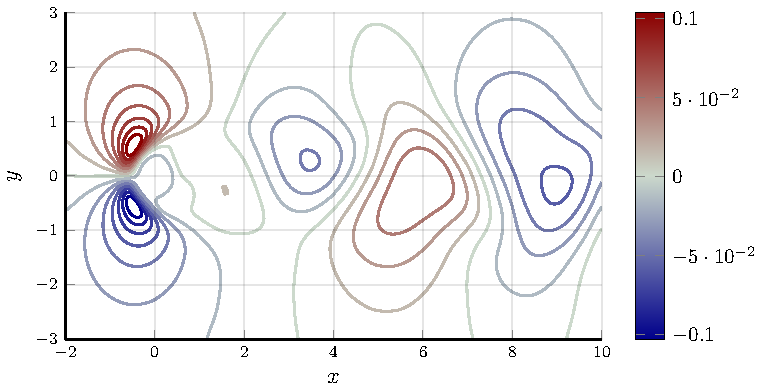
\includegraphics[width=\columnwidth]{./figures/yvel}} \\
    \subfloat[pressure]{\label{pressure}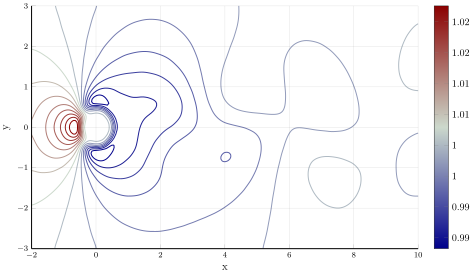
\includegraphics[width=\columnwidth]{./figures/pressure}}
    \caption{Global caption that can reference \ref{sublable1} and \ref{sublable2}}
    \label{fig:ns_data}
    \vskip -0.2in
\end{figure}

\begin{figure}
\vskip -0.15in
\centering
    \begin{equation*}
        \begin{split}
          \mathbb{R} &\mapsto u \quad | \quad v \quad | \quad p \\
          \mathbb{R} &\mapsto \frac{d\mathbb{R}}{dx} \quad \left| \quad \frac{d\mathbb{R}}{dy} \right. \\
          \mathbb{R} &\mapsto \mathbb{R} \times \mathbb{R}
        \end{split}
    \end{equation*}
    \vskip -0.15in
    \caption{Grammar used for the Navier-Stokes equations}
    \label{fig:nsgrammar}
    \vskip -.15in
\end{figure}

SIEO was performed on the the vortex shedding data with the adjusted $R^2$ loss function and $\alpha = 0.2 $. The algorithm found equations \ref{eqn:xmom} and \ref{eqn:ymom} to explain the unsteady Navier-Stokes data
\begin{align}
\label{eqn:xmom}
    \frac{\partial u}{\partial t} &= {\theta_x}_1 \frac{\partial}{\partial y} (u v) + {\theta_x}_2 v \frac{\partial u}{\partial y} + {\theta_x}_3 \frac{\partial p}{\partial y} + {\theta_x}_4 \frac{\partial^2 u}{\partial y^2} \\
\label{eqn:ymom}
    \frac{\partial v}{\partial t} &= {\theta_y}_1 u \frac{\partial v}{\partial x} (u v) + {\theta_y}_2 v \frac{\partial v}{\partial y} + {\theta_y}_3 \frac{\partial p}{\partial y}
\end{align}
Note that the first equation requires the substitution $\partial v /\partial y = - \partial u / \partial x $ (from the continuity equation) to transform it to the more well-known form of the $x$-momentum equation. Also note the absence of the viscous terms $\partial^2 u / \partial x^2$, $\partial^2 v / \partial x^2$, and $\partial^2 v / \partial y^2$. These terms are not included because in this particular fluid flow they are much smaller in magnitude than the other terms in the governing equation. This shows that for SIEO to identify a process, that process must be sufficiently active in the data collected. 

The ratios of the model coefficients were compared to get a sense of the error in the model parameters. The results are shown in table \ref{tab:ns_data}. In general, the model parameter error is very small and the discovered equations could be used for prediction or control of other similar types of flow field (i.e. those that don't have significant contributions from the viscous terms).

\begin{table}[t]
\caption{Error in Navier-Stokes Coefficients}
\label{tab:ns_data}
\vskip 0.15in
\begin{center}
\begin{small}
\begin{sc}
\begin{tabular}{lccccr}
\toprule
Parameter & Error \\
\midrule
${\theta_x}_2 / {\theta_x}_1 $ & 2.87 \% \\
${\theta_x}_3 / {\theta_x}_1 $ & 1.00 \% \\
${\theta_x}_4 / {\theta_x}_1 $ & 2.53 \% \\
${\theta_y}_2 / {\theta_x}_1 $ & 8.47 \% \\
${\theta_y}_3 / {\theta_x}_1 $ & 0.92 \% \\
\bottomrule
\end{tabular}
\end{sc}
\end{small}
\end{center}
\vskip -0.1in
\end{table}

\subsection{Exact Koopman Eigenfunction Discovery}
\label{exactdiscovery}
A simple nonlinear ODE with an easily found, and finite-dimensional Koopman eigenfunctions is given by [Brunton citation]
\begin{equation}
\begin{split}
  \label{simplekoopman}
\frac{dx}{dt} = \mu x \\
\frac{dy}{dt} = \lambda(y - x^2)
\end{split}
\end{equation}
The state-space transformation
\begin{equation}
    \label{eqn:exacttransform}
\begin{bmatrix}
x\\
y
\end{bmatrix} \Rightarrow \begin{bmatrix}
x \\
y \\
x^2
\end{bmatrix}
\end{equation}
linearizes equation \ref{simplekoopman} to
\begin{equation}
    \label{eqn:koopmanop}
\frac{d}{dt} \begin{bmatrix}
x \\
y \\
x^2
\end{bmatrix} = \begin{bmatrix}
\mu & 0 & 0 \\
0 & \lambda & -\lambda \\
0 & 0 & 2 \mu
\end{bmatrix} \begin{bmatrix}
x \\
y \\
x^2
\end{bmatrix}
\end{equation}

To test the discovery of exact Koopman operators, data from the system (\ref{simplekoopman}) was collected data for many initial conditions. The initial data is stored in a vector $\vec{x}^0$, then the solution is integrated forward one timestep and the result is stored in another vector $\vec{x}^1$. SIEO was then applied with the average sum of squares loss function $l_k$. The goal was to find a state-inclusive Koopman operator so the loss function was modified to penalize the absence of the primary state variables $x$ and $y$. The function-rich grammar in figure \ref{fig:odegrammar} was used as input (exchanging ($\theta$, $\omega$) for ($x$, $y$)). The correct Koopman transformation was discovered (equation \ref{eqn:exacttransform}) and the Koopman operator (equation \ref{eqn:koopmanop}) was recovered to within machine precision.







\subsection{Approximate Koopman Eigenfunction Discovery of Nonlinear Pendulum}
One of the simplest nonlinear ODEs without a known Koopman operator, is a simple pendulum swinging at large angles. The equation of motion a pendulum is given by
\[ \frac{d^2 \theta}{d t^2} + \sin \theta = 0 \]
This equation can be converted to a system of nonlinear first-order ODEs given by
\begin{align*}
\frac{d\theta}{dt} &= \omega \\
\frac{d\omega}{dt} &= -\sin \theta
\end{align*}


\begin{figure}
\vskip -0.15in
\centering
\begin{equation*}
    \begin{split}
        \mathbb{R} &\mapsto \theta \quad | \quad \omega \\
        \mathbb{R} &\mapsto \mathbb{R} \times \mathbb{R} \\
        \mathbb{R} &\mapsto \sin (\mathbb{G} \times \mathbb{R}) \quad | \quad \sin (\mathbb{G} \times \mathbb{R} + \mathbb{G}) \\
        \mathbb{R} &\mapsto {\rm exp}(\mathbb{G} \times \mathbb{R}) \\
        \mathbb{R} &\mapsto 1 / (1 + {\rm exp}(-\mathbb{G} \times \mathbb{R})) \\
        \mathbb{R} &\mapsto {\rm exp}(-(\mathbb{R}-\mathbb{G})^2/\mathbb{G}) \\
        \mathbb{R} &\mapsto {\rm imag}(\mathbb{R}^\mathbb{G}) \\
        \mathbb{R} &\mapsto {\rm real}(\mathbb{R}^\mathbb{G}) \\
        \mathbb{G} &\mapsto -\mathbb{G} \quad | \quad \mathbb{G}+\mathbb{G} \quad | \quad \mathbb{G}/\mathbb{G} \\
        \mathbb{G} &\mapsto {\rm logspace(-5, 2, 20)}
    \end{split}
\end{equation*}
    \vskip -0.15in
    \caption{Grammar used for both nonlinear ODEs}
    \label{fig:odegrammar}
    \vskip -.15in
\end{figure}


\todo{section on methods}
In order to generate training data, the system was integrated forward in time from a starting position $(\theta_0, \omega_0) = (\pi/2, 0)$ until $T=10$. Koopman operator was approximated by SIEO using the average sum of squares loss function with the same state-inclusive penalty described in section \ref{exactdiscovery}. The function-rich grammar shown in figure \ref{fig:odegrammar} was used as the input. The resulting expression with $24$ features was then compared to a linearized version of the equation with only the primary state variables. Both linear models were initialized at $(\theta_0, \omega_0) = (\pi/2, 0)$ and were allowed to evolve forward in time past the training period. The error between the linear model and the exact solution for each model is shown in figure \ref{fig:pendulum}.

The figure shows that the linear model with more nonlinear features has significantly lower average error then the linear model with only the two state variables. Additionally, the error more slowly for the Koopman approximation. This shows that it is possible to improve linearizations of nonlinear model by using expression optimization to approximate the Koopman eigenfunctions of the system.

\begin{figure}
\vskip 0.2in
\begin{center}
\centerline{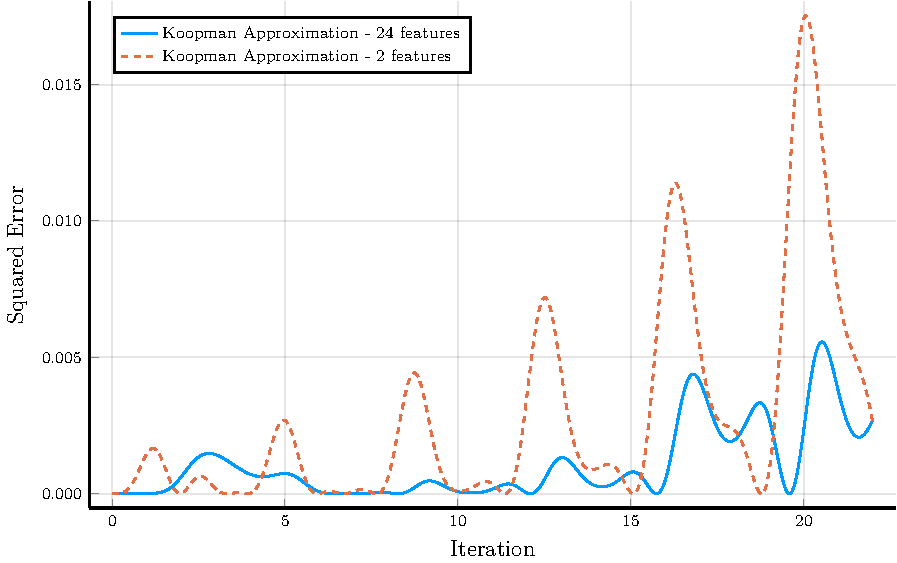
\includegraphics[width=\columnwidth]{./figures/pendulum}}
\caption{Error in the nonlinear pendulum for the simplest linear model and linear model with more nonlinear features}
\label{fig:pendulum}
\end{center}
\vskip -0.2in
\end{figure}

\section{Conclusions}
\label{conclusion}

\begin{itemize}
    \item Robustness in finding correct features in the presence of noise and limited data make the resulting model very generalizeable
    \item It can seach through a vast number of possible features and mappings -- even in problems with multiple state variables and multiple dimenions
    \item Presesnts a new way of finding exact and approximate Koopman operators
\end{itemize}

\todo{Summarize and conclude}



% Acknowledgements should only appear in the accepted version.
% \section*{Acknowledgements}

% In the unusual situation where you want a paper to appear in the
% references without citing it in the main text, use \nocite

% \bibliography{example_paper}
\bibliographystyle{icml2019}


\end{document}


% This document was modified from the file originally made available by
% Pat Langley and Andrea Danyluk for ICML-2K. This version was created
% by Iain Murray in 2018, and modified by Alexandre Bouchard in
% 2019. Previous contributors include Dan Roy, Lise Getoor and Tobias
% Scheffer, which was slightly modified from the 2010 version by
% Thorsten Joachims & Johannes Fuernkranz, slightly modified from the
% 2009 version by Kiri Wagstaff and Sam Roweis's 2008 version, which is
% slightly modified from Prasad Tadepalli's 2007 version which is a
% lightly changed version of the previous year's version by Andrew
% Moore, which was in turn edited from those of Kristian Kersting and
% Codrina Lauth. Alex Smola contributed to the algorithmic style files.
